\documentclass[twoside]{book}

% Packages required by doxygen
\usepackage{fixltx2e}
\usepackage{calc}
\usepackage{doxygen}
\usepackage[export]{adjustbox} % also loads graphicx
\usepackage{graphicx}
\usepackage[utf8]{inputenc}
\usepackage{makeidx}
\usepackage{multicol}
\usepackage{multirow}
\PassOptionsToPackage{warn}{textcomp}
\usepackage{textcomp}
\usepackage[nointegrals]{wasysym}
\usepackage[table]{xcolor}

% NLS support packages
\usepackage{polski}
\usepackage[T1]{fontenc}

% Font selection
\usepackage[T1]{fontenc}
\usepackage[scaled=.90]{helvet}
\usepackage{courier}
\usepackage{amssymb}
\usepackage{sectsty}
\renewcommand{\familydefault}{\sfdefault}
\allsectionsfont{%
  \fontseries{bc}\selectfont%
  \color{darkgray}%
}
\renewcommand{\DoxyLabelFont}{%
  \fontseries{bc}\selectfont%
  \color{darkgray}%
}
\newcommand{\+}{\discretionary{\mbox{\scriptsize$\hookleftarrow$}}{}{}}

% Page & text layout
\usepackage{geometry}
\geometry{%
  a4paper,%
  top=2.5cm,%
  bottom=2.5cm,%
  left=2.5cm,%
  right=2.5cm%
}
\tolerance=750
\hfuzz=15pt
\hbadness=750
\setlength{\emergencystretch}{15pt}
\setlength{\parindent}{0cm}
\setlength{\parskip}{3ex plus 2ex minus 2ex}
\makeatletter
\renewcommand{\paragraph}{%
  \@startsection{paragraph}{4}{0ex}{-1.0ex}{1.0ex}{%
    \normalfont\normalsize\bfseries\SS@parafont%
  }%
}
\renewcommand{\subparagraph}{%
  \@startsection{subparagraph}{5}{0ex}{-1.0ex}{1.0ex}{%
    \normalfont\normalsize\bfseries\SS@subparafont%
  }%
}
\makeatother

% Headers & footers
\usepackage{fancyhdr}
\pagestyle{fancyplain}
\fancyhead[LE]{\fancyplain{}{\bfseries\thepage}}
\fancyhead[CE]{\fancyplain{}{}}
\fancyhead[RE]{\fancyplain{}{\bfseries\leftmark}}
\fancyhead[LO]{\fancyplain{}{\bfseries\rightmark}}
\fancyhead[CO]{\fancyplain{}{}}
\fancyhead[RO]{\fancyplain{}{\bfseries\thepage}}
\fancyfoot[LE]{\fancyplain{}{}}
\fancyfoot[CE]{\fancyplain{}{}}
\fancyfoot[RE]{\fancyplain{}{\bfseries\scriptsize Wygenerowano przez Doxygen }}
\fancyfoot[LO]{\fancyplain{}{\bfseries\scriptsize Wygenerowano przez Doxygen }}
\fancyfoot[CO]{\fancyplain{}{}}
\fancyfoot[RO]{\fancyplain{}{}}
\renewcommand{\footrulewidth}{0.4pt}
\renewcommand{\chaptermark}[1]{%
  \markboth{#1}{}%
}
\renewcommand{\sectionmark}[1]{%
  \markright{\thesection\ #1}%
}

% Indices & bibliography
\usepackage{natbib}
\usepackage[titles]{tocloft}
\setcounter{tocdepth}{3}
\setcounter{secnumdepth}{5}
\makeindex

% Hyperlinks (required, but should be loaded last)
\usepackage{ifpdf}
\ifpdf
  \usepackage[pdftex,pagebackref=true]{hyperref}
\else
  \usepackage[ps2pdf,pagebackref=true]{hyperref}
\fi
\hypersetup{%
  colorlinks=true,%
  linkcolor=blue,%
  citecolor=blue,%
  unicode%
}

% Custom commands
\newcommand{\clearemptydoublepage}{%
  \newpage{\pagestyle{empty}\cleardoublepage}%
}

\usepackage{caption}
\captionsetup{labelsep=space,justification=centering,font={bf},singlelinecheck=off,skip=4pt,position=top}

%===== C O N T E N T S =====

\begin{document}

% Titlepage & ToC
\hypersetup{pageanchor=false,
             bookmarksnumbered=true,
             pdfencoding=unicode
            }
\pagenumbering{roman}
\begin{titlepage}
\vspace*{7cm}
\begin{center}%
{\Large M\+I\+LL }\\
\vspace*{1cm}
{\large Wygenerowano przez Doxygen 1.8.11}\\
\end{center}
\end{titlepage}
\clearemptydoublepage
\tableofcontents
\clearemptydoublepage
\pagenumbering{arabic}
\hypersetup{pageanchor=true}

%--- Begin generated contents ---
\chapter{Indeks klas}
\section{Lista klas}
Tutaj znajdują się klasy, struktury, unie i interfejsy wraz z ich krótkimi opisami\+:\begin{DoxyCompactList}
\item\contentsline{section}{\hyperlink{structboard}{board} \\*Struktura planszy w grze }{\pageref{structboard}}{}
\item\contentsline{section}{\hyperlink{structmy__button}{my\+\_\+button} \\*Struktuja guzika z obrazkiem }{\pageref{structmy__button}}{}
\item\contentsline{section}{\hyperlink{structpipes}{pipes} }{\pageref{structpipes}}{}
\item\contentsline{section}{\hyperlink{structplayer}{player} \\*Struktuja gracza }{\pageref{structplayer}}{}
\end{DoxyCompactList}

\chapter{Dokumentacja klas}
\hypertarget{structboard}{}\section{Dokumentacja klasy board}
\label{structboard}\index{board@{board}}


Struktura planszy w grze.  




{\ttfamily \#include $<$board.\+h$>$}



Diagram współpracy dla board\+:
\nopagebreak
\begin{figure}[H]
\begin{center}
\leavevmode
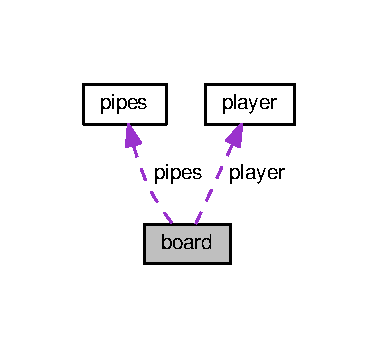
\includegraphics[width=182pt]{structboard__coll__graph}
\end{center}
\end{figure}
\subsection*{Atrybuty publiczne}
\begin{DoxyCompactItemize}
\item 
int {\bfseries tab} \mbox{[}7\mbox{]}\mbox{[}7\mbox{]}\hypertarget{structboard_a1fec2ea31b5f84e51e480ee7124e21dd}{}\label{structboard_a1fec2ea31b5f84e51e480ee7124e21dd}

\item 
unsigned int {\bfseries state}\hypertarget{structboard_a4bdf7e0cd3652096d965adc19bd8832c}{}\label{structboard_a4bdf7e0cd3652096d965adc19bd8832c}

\item 
unsigned int {\bfseries turn}\hypertarget{structboard_a5253e1b4538cace8c76b0ea1ceded4b3}{}\label{structboard_a5253e1b4538cace8c76b0ea1ceded4b3}

\item 
int {\bfseries update}\hypertarget{structboard_a95e163830d33ed01b87452d250919820}{}\label{structboard_a95e163830d33ed01b87452d250919820}

\item 
\hyperlink{structplayer}{Player} {\bfseries player} \mbox{[}2\mbox{]}\hypertarget{structboard_a130c34c1f03cd17f11fcf81083526922}{}\label{structboard_a130c34c1f03cd17f11fcf81083526922}

\item 
char $\ast$ {\bfseries error}\hypertarget{structboard_a94b1302fd63bb9b017d0a9af33840bb3}{}\label{structboard_a94b1302fd63bb9b017d0a9af33840bb3}

\item 
int {\bfseries last\+\_\+x}\hypertarget{structboard_a227249cb7c1b1379e9dd2d5c5b652216}{}\label{structboard_a227249cb7c1b1379e9dd2d5c5b652216}

\item 
int {\bfseries last\+\_\+y}\hypertarget{structboard_a2f14ddf3a3a7b4e145578bbcfc9a73ee}{}\label{structboard_a2f14ddf3a3a7b4e145578bbcfc9a73ee}

\item 
Gtk\+Widget $\ast$ {\bfseries info}\hypertarget{structboard_adf62f066ab1743df1e6c44550c70f9e0}{}\label{structboard_adf62f066ab1743df1e6c44550c70f9e0}

\item 
Gtk\+Widget $\ast$ {\bfseries score}\hypertarget{structboard_a05d95ee8ddfc53f3358d3a8e45b7b65b}{}\label{structboard_a05d95ee8ddfc53f3358d3a8e45b7b65b}

\item 
\hyperlink{structpipes}{Pipes\+Ptr} {\bfseries pipes}\hypertarget{structboard_aef3b34c8c45a5d639ea1aba23f94b912}{}\label{structboard_aef3b34c8c45a5d639ea1aba23f94b912}

\item 
int {\bfseries color}\hypertarget{structboard_a8ab755e152d7db496709368179df93fa}{}\label{structboard_a8ab755e152d7db496709368179df93fa}

\end{DoxyCompactItemize}


\subsection{Opis szczegółowy}
Struktura planszy w grze. 

Dokumentacja dla tej klasy została wygenerowana z pliku\+:\begin{DoxyCompactItemize}
\item 
board.\+h\end{DoxyCompactItemize}

\hypertarget{structmy__button}{}\section{Dokumentacja klasy my\+\_\+button}
\label{structmy__button}\index{my\+\_\+button@{my\+\_\+button}}


Struktuja guzika z obrazkiem.  




{\ttfamily \#include $<$my\+\_\+button.\+h$>$}



Diagram współpracy dla my\+\_\+button\+:
\nopagebreak
\begin{figure}[H]
\begin{center}
\leavevmode
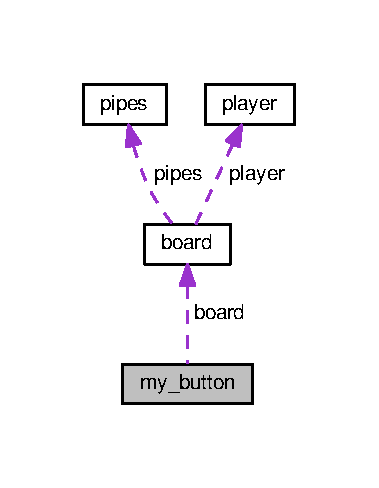
\includegraphics[width=182pt]{structmy__button__coll__graph}
\end{center}
\end{figure}
\subsection*{Atrybuty publiczne}
\begin{DoxyCompactItemize}
\item 
char $\ast$ {\bfseries assets} \mbox{[}3\mbox{]}\hypertarget{structmy__button_a3a9778fafcb88866f6a084aac82055a2}{}\label{structmy__button_a3a9778fafcb88866f6a084aac82055a2}

\item 
\hyperlink{structboard}{Board} {\bfseries board}\hypertarget{structmy__button_a696a9280a90d1b7f2bb041832c1eafe4}{}\label{structmy__button_a696a9280a90d1b7f2bb041832c1eafe4}

\item 
Gtk\+Widget $\ast$ {\bfseries event\+\_\+box}\hypertarget{structmy__button_a30176d0d65c9e03e19d912bce69b3240}{}\label{structmy__button_a30176d0d65c9e03e19d912bce69b3240}

\item 
Gtk\+Widget $\ast$ {\bfseries image}\hypertarget{structmy__button_ac0d07c21d699515ebf2626fa6e7ede47}{}\label{structmy__button_ac0d07c21d699515ebf2626fa6e7ede47}

\item 
int {\bfseries x}\hypertarget{structmy__button_a6bd896eb399fe422ae03e4f2eaad53af}{}\label{structmy__button_a6bd896eb399fe422ae03e4f2eaad53af}

\item 
int {\bfseries y}\hypertarget{structmy__button_a32323eb674397182f5ec463ef52fef83}{}\label{structmy__button_a32323eb674397182f5ec463ef52fef83}

\item 
int {\bfseries state}\hypertarget{structmy__button_ade000e7dc35bbfbc7def62c34fe731a3}{}\label{structmy__button_ade000e7dc35bbfbc7def62c34fe731a3}

\end{DoxyCompactItemize}


\subsection{Opis szczegółowy}
Struktuja guzika z obrazkiem. 

Dokumentacja dla tej klasy została wygenerowana z pliku\+:\begin{DoxyCompactItemize}
\item 
my\+\_\+button.\+h\end{DoxyCompactItemize}

\hypertarget{structpipes}{}\section{Dokumentacja klasy pipes}
\label{structpipes}\index{pipes@{pipes}}


{\ttfamily \#include $<$fifo.\+h$>$}

\subsection*{Atrybuty publiczne}
\begin{DoxyCompactItemize}
\item 
F\+I\+LE $\ast$ {\bfseries fifo\+\_\+in}\hypertarget{structpipes_afa1c912838d89882e1112aa54825c95d}{}\label{structpipes_afa1c912838d89882e1112aa54825c95d}

\item 
F\+I\+LE $\ast$ {\bfseries fifo\+\_\+out}\hypertarget{structpipes_a872ae4c7721473f4d9cc5af6f6f5426a}{}\label{structpipes_a872ae4c7721473f4d9cc5af6f6f5426a}

\item 
int {\bfseries isA}\hypertarget{structpipes_ab28a99ff248f3d282ac64846cbf82d74}{}\label{structpipes_ab28a99ff248f3d282ac64846cbf82d74}

\end{DoxyCompactItemize}


\subsection{Opis szczegółowy}
\begin{DoxyAuthor}{Autor}
Marek Piotrów 
\end{DoxyAuthor}


Dokumentacja dla tej klasy została wygenerowana z pliku\+:\begin{DoxyCompactItemize}
\item 
fifo.\+c\end{DoxyCompactItemize}

\hypertarget{structplayer}{}\section{Dokumentacja klasy player}
\label{structplayer}\index{player@{player}}


Struktuja gracza.  




{\ttfamily \#include $<$player.\+h$>$}

\subsection*{Atrybuty publiczne}
\begin{DoxyCompactItemize}
\item 
int {\bfseries pawns}\hypertarget{structplayer_ac324cb782faa8689b1516ba54f6dfae3}{}\label{structplayer_ac324cb782faa8689b1516ba54f6dfae3}

\item 
int {\bfseries in\+\_\+stash}\hypertarget{structplayer_ab649f20ffcb98bd133d93f7950f3e4f3}{}\label{structplayer_ab649f20ffcb98bd133d93f7950f3e4f3}

\item 
char $\ast$ {\bfseries name}\hypertarget{structplayer_a27bb715521eb5315f3b6238d11061817}{}\label{structplayer_a27bb715521eb5315f3b6238d11061817}

\end{DoxyCompactItemize}


\subsection{Opis szczegółowy}
Struktuja gracza. 

Dokumentacja dla tej klasy została wygenerowana z pliku\+:\begin{DoxyCompactItemize}
\item 
player.\+h\end{DoxyCompactItemize}

%--- End generated contents ---

% Index
\backmatter
\newpage
\phantomsection
\clearemptydoublepage
\addcontentsline{toc}{chapter}{Indeks}
\printindex

\end{document}
